\chapter{Campo magnetico}

Il campo magnetico è una grandezza vettoriale che descrive l'interazione tra corpi dotati di natura magnetica; questa grandezza di misura in Tesla [T] e solitamente si indica con la lettera B.
I fenomeni di magnetismo non sono altro che la manifestazione tra cariche elettriche in movimento ordinato, come quello formato dalle cariche elettriche che attraversano un filo.
\paragraph{}
Ad esempio in un magnete naturale tutte le microscopiche correnti locali
generate dagli elettroni che ruotano tutti alla stessa maniera si sommano per
formare a livello macroscopico il campo magnetico che abbiamo imparato ad
individuare.

Invece un pezzo di ferro qualsiasi non è magnetico in quanto le correnti
microscopiche che sono presenti al suo interno in media tendono ad annullarsi in
quanto gli elettroni si muovono disordinatamente in tutte le direzioni dello spazio
annullando l'effetto dei micro campi magnetici che ognuno di essi genera.

\section{Verso del campo magnetico}
Il verso del campo magnetico dipende dal verso della corrente e segue la legge della mano destra. L'immagine di seguito vale più di molte parole.

\begin{figure}[H]
    \centering
    \begin{tikzpicture}[scale = 0.7]
      \coordinate (O) at (1.1,0.2); % ORIGIN
      \coordinate (WT) at ( 2.9,-1.1); % WRIST TOP
      \coordinate (T1) at ( 2.3, 0.7); % THUMB
      \coordinate (T2) at ( 1.75, 2.3);
      \coordinate (T3) at ( 2.0, 3.1);
      \coordinate (T4) at (1.38, 3.15);
      \coordinate (T5) at ( 0.9, 2.3);
      \coordinate (T6) at ( 0.85, 1.2);
      \coordinate (T7) at ( 0.9, 0.2);
      \coordinate (I1) at (-0.1, 1.4); % INDEX
      \coordinate (I2) at (-1.3, 1.2);
      \coordinate (I3) at (-1.6, 0.5);
      \coordinate (I4) at (-0.7,-0.4);
      \coordinate (I5) at ( 0.1,-0.6);
      \coordinate (I6) at ( 0.1,-0.05);
      \coordinate (I7) at (-0.4,0.19);
      \coordinate (I8) at (-1.0, 0.9);
      \coordinate (M1) at (-1.8,-0.1); % MIDDLE
      %\coordinate (M2) at (-0.5,-0.7);
      \coordinate (M2) at (-0.8,-1.0);
      \coordinate (M3) at ( 0.1,-1.15);
      \coordinate (R1) at (-1.8,-0.8); % RING
      \coordinate (R2) at (-0.9,-1.6);
      \coordinate (R3) at (-0.0,-1.7);
      \coordinate (R4) at ( 0.0,-1.1);
      \coordinate (P1) at (-1.9,-1.4); % PINKY
      \coordinate (P2) at (-1.0,-2.1);
      \coordinate (P3) at (-0.3,-2.15);
      \coordinate (W1) at ( 0.4,-2.9); % WRIST BOTTOM
      \coordinate (W2) at ( 1.6,-3.5);
      
      % HAND
      \fill[brownskin]
        (WT) -- (T6) -- (I2) -- (P2) -- (W1) -- (W2) to[out=25,in=-90] cycle;
      \draw[fill=brownskin]
        (WT) to[out=120,in=-60] % THUMB
        (T1) to[out=120,in=-90]
        (T2) to[out=80,in=-110]
        (T3) to[out=80,in=50,looseness=1.5] % tip
        (T4) to[out=-130,in=80]
        (T5) to[out=-100,in=70]
        (T6) to[out=-100,in=100]
        (T7)
        (T6) -- % INDEX
        (I1) to[out=170,in=15]
        (I2) to[out=-165,in=140,looseness=1.2] % knuckle
        (I3) to[out=-60,in=140,looseness=0.8]
        (I4) to[out=-40,in=180,looseness=0.4]
        (I5) to[out=20,in=-30,looseness=1.3] % tip
        (I6) to[out=150,in=-20]
        (I7) to[out=120,in=-30]
        (I8)
        (I7) to[out=160,in=-15]++ (162:0.18)
        (I3) to[out=180,in=140,looseness=0.9] % MIDDLE
        (M1) to[out=-60,in=150,looseness=0.8]
        (M2) to[out=-30,in=175,looseness=0.4]
        (M3) to[out=-5,in=-15,looseness=1.5] % tip
        (I5)
        (M1) to[out=-130,in=135,looseness=1.2] % knuckle
        (R1) to[out=-45,in=160,looseness=0.9]
        (R2) to[out=-20,in=180,looseness=0.4]
        (R3) to[out=0,in=-15,looseness=1.5] % tip
        (M3)
        (R1) to[out=-150,in=130] % PINKY
        (P1) to[out=-50,in=165]
        (P2) to[out=-15,in=180,looseness=0.9]
        (P3) to[out=0,in=-35,looseness=1.5] % tip
        (R3)
        (P2) to[out=-35,in=145] % WRIST
        (W1) to[out=-35,in=160]
        (W2);
      
      % FOLDS
      \draw[very thin] (T5)++(-80:0.3) to[out=40,in=180]++ (25:0.45); % THUMB
      \draw[very thin] (I4)++(135:0.1) to[out=100,in=-110]++ (80:0.4); % INDEX
      \draw[very thin] (M2)++(130:0.1) to[out=100,in=-110]++ (80:0.4); % MIDDLE
      \draw[very thin] (R2)++(140:0.1) to[out=95,in=-110]++ (80:0.4); % RING
      \draw[very thin] (P2)++(145:0.1) to[out=95,in=-110]++ (85:0.4); % PINKY
      \draw[very thin] (I8)++(-33:0.55) to[out=50,in=-90]++ (70:0.6); % PALM
      \draw[very thin] (I7)++(-5:0.2) to[out=70,in=-80]++ (80:1.1); % PALM
      \draw[very thin] (W2)++(70:1.4) to[out=-175,in=-40]++ (160:1.4); % PALM
      
      % VECTORS
      \def\Rx{2.4}
      \def\Ry{0.7}
      \draw[very thick]
        (O)++(-108.5:3.6) --++ (78:7.1);
      \draw[current,very thick]
        (O)++(106:1.2) --++ (78:2.1)
        node[midway,left,scale=1.5] {$\vb{I}$};
      \draw[BField,rotate=-15]
        (O)++(-250:{\Rx} and {\Ry}) arc (-250:-80:{\Rx} and {\Ry})
        node[below=1,scale=1.5] {$\vb{B}$};
      
    \end{tikzpicture}
    \caption{Verso del campo magnetico}
    \label{fig:versoCampoiMagnetico}
\end{figure}

\section{Legge di Gauss per il campo magnetico}

\begin{equation}
    \oint_S \vec{B}\cdot d\vec{S} = 0
\end{equation}

Questa formula esprime la solenoidalità del campo magnetico: si definisce il campo magnetico solenoidale il flusso attraverso una qualsiasi superficie chiusa è nullo.
Questa è meno utilizzata rispetto alla legge di Gauss per il campo elettrico.

\section{Legge di Ampère}
\begin{equation}
    \oint_L \vec{B}\cdot d\vec{L} = \mu_0I
\end{equation}
Questa formula è molto simile alla formula per calcolare il flusso del campo magnetico e essa indica che l'integrale di linea su una linea chiusa, lo stesso metodo che si utilizza per calcolare il lavoro su una linea chiusa, e risulta uguale ad una costante $\mu_0$ moltiplicato per la corrente che sta trapassando quella linea chiusa. Per trapassare si intende che la corrente sta passando per una superficie arbitraria appoggiata alla linea chiusa, si pensi sempre ad una bolla di sapone.
\paragraph{}
La costante $\mu_0 $vale:
\begin{equation*}
    \mu_0 = 4\pi 10^{-7}
\end{equation*}

Questa formula non è completa, a completarla sarà successivamente Maxwell, il quale rende il sistema delle quattro equazioni coerenti e in grado di studiare tutti i fenomeni elettromagentici.

\section{Campo magnetico filo infinito}
\begin{figure}[H]
    \centering
    \begin{tikzpicture}[z={(0.8,0.28)},x={(0.58,-0.45)}]
      \def\L{6}
      \def\W{0.10}
      \def\R{0.9}
      \def\ang{-35}
      \def\scale{1.3}
      \def\NB{5}
      \coordinate (O) at (0,0,0);
      %\draw (0,0,0) -- (2,0,0);
      %\draw (0,0,0) -- (0,0,2);
      
      % B FIELD BACK
      \foreach \i [evaluate={\x=(\i-\NB/2-0.5)*\L/\NB;}] in {1,...,\NB}{
        %\draw[BField,-] (0,0,\x)++(\ang+1:\R) arc (\ang+1:\ang-181:\R);
        \draw[BFieldLine=1] (0,0,\x)++(\ang+1:\R) arc (\ang+1:\ang-181:\R) --++ (65:0.001*\R);
      }
      
      % WIRE
      \draw[metal] (0,0,-\L/2)++(120:\W/2) --++ (0,0,\L) arc (120:-60:\W/2) --++ (0,0,-\L) arc (-60:120:\W/2);
      \draw[metal] (0,0,-\L/2) circle (\W/2);
      \draw[current] (0.12*\R,-0.12*\R,0.4*\L) --++ (0,0,0.2*\L) node[below=2,right] {$I = 2A$};
      
      % B FIELD FRONT
      \foreach \i [evaluate={\x=(\i-\NB/2-0.5)*\L/\NB;}] in {1,...,\NB}{
        %\draw[BFieldLine=1] (0,0,\x)++(\ang+180:\R) arc (\ang+180:\ang:\R) --++ (-116:0.001*\R);
        \draw[BField,-] (0,0,\x)++(\ang+180:\R) arc (\ang+180:\ang:\R);
      }
      \node[Bcol] at (-0.9*\R,0.9*\R,-0.25*\L) {$\vb{B}$}; %++(140:1.3*\R)
      
    \end{tikzpicture}
    \caption{Campo magnetico filo infinito}
    \label{fig:campoEletFiloInf}
\end{figure}

In ogni punto la corrente sta trapassando un disco di raggio $r$, sul quale volendo si potrebbe spingere la superficie intera verso l'esterno, come se soffiassimo per creare una bolla di sapone, e il campo magnetico non cambia.

\paragraph{}
Sapendo che la corrente è $2A$ possiamo calcolare il risultato dell'integrale di linea della legge di Ampère:

\begin{equation*}
    \mu_0I = 4\pi 10^{-7}2 = 8\pi 10^{-7}
\end{equation*}


Dunque l'integrale sulla circonferenza risulta essere:

\begin{equation*}
    \oint_S \vec{B}\cdot d\vec{l} = \mu_0I
\end{equation*}
Essendo $\vec{B}$ costante, perché tangente alla circonferenza si può portare fuori dall'integrale:
\begin{equation*}
    B\oint_S dl = \mu_0I
\end{equation*}
L'integrale risulta essere una circonferenza di un cerchio avente raggio $r$:
\begin{equation}
    B2\pi r = \mu_0I
\end{equation}

\begin{equation*}
    B = \frac{\mu_0I}{2\pi r}
\end{equation*}


\begin{figure}[H]
    \centering
    \begin{tikzpicture}
      \def\R{0.66}
      \def\RB{1.5}
      \def\RA{1.4}
      \def\RAin{0.77*\R}
      \def\NB{2}
      
      % AXIS
      \draw[metal] (0,0) circle (\R);
      \draw[->] (0,0) -- (50:\RA) node[midway,right=8,above left=2] {$r$};
      
      % AMPERE LOOP
      \draw[Ampcurve={0.52}] (0,0) circle (\RA);
      \draw[Ampcurve={1}] (-175:\RAin) arc (-175:185:\RAin) --++ (-92:0.01);
      \node[Ampcol,right] at (182:\RA) {$\dd\vb*{\ell}$};
      
      % CURRENT
      \draw[->] (0,0) -- (-76:\R) node[midway,left=-1,scale=0.8] {$R$};
      \pic[scale=0.81] at (0,0) {Bout={Icol}};
      \node[Icol] at (0:0.4*\R) {$I$};
      
      % MAGNETIC FIELDLINES
      %\foreach \i [evaluate={\r=\RB*\i)}] in {1,...,\NB}{
      \draw[BFieldLine={0.49}] (0,0) circle (\RB);
      %}
      \node[Bcol,left] at (174:\RB) {$\vb{B}$};
      
    \end{tikzpicture}
    \caption{Sezione del filo vista dall'alto}
    \label{fig:sezioneFiloMagnetico}
\end{figure}


\section{Campo magnetico in un solenoide infinito}

\begin{figure}[H]
    \centering
    \contourlength{1.0pt}
    \begin{tikzpicture}
      \message{Loop with Ampere's law start. ^^J}
      \def\R{1}
      \def\N{12}
      \def\NB{3}
      \def\L{6}
      \def\t{0.20*\R}
      \def\w{\L/(\N-1)}
      %\draw[current] (-0.6*\R,-0.01*\R) arc (-94:-86:{0.6*\R/sin(4)})
      %  node[midway,below=0.6] {\contour{white}{$I$}};
      
      % WIRE BACK
      \foreach \i [evaluate={\x=-\L/2+(\i-1)*\w; \ang=atan(4*\R/(\w));}] in {1,...,\N}{
        \ifthenelse{\i<\N}{
          \draw[lightmetal]
            ({\x+\w/2},-\R)++(\ang+90:\t/2) to[out=\ang+5,in=\ang-185]++ (\ang:2.02*\R) -- ({\x+\w},\R)
                                            --++ (\ang-90:\t/2) to[out=\ang-185,in=\ang+5]++ (\ang-180:2.02*\R) -- cycle;
        }{}
      }
      
      % MAGNETIC FIELDLINES
      \foreach \i [evaluate={\y=(\i-\NB/2-0.5)*1.4*\R/\NB}] in {1,...,\NB}{
          \draw[BFieldLine={0.505}] (-0.55*\L,\y) -- (0.62*\L,\y);
      }
      \node[Bcol] at (0.61*\L,0.76*\R) {$\vb{B}$};
      
      % AMPERE's LOOP
      \draw[Ampcol]
        (-0.27*\L,0.6*\R) -| (0.27*\L,1.5*\R) -| cycle;
      \draw[Ampcurve={0.54}]
        (-0.27*\L,0.6*\R) -- (0.27*\L,0.6*\R);
      \draw[Ampcurve={0.68}]
        ( 0.27*\L,0.6*\R) -- (0.27*\L,1.5*\R);
      \draw[Ampcurve={0.55}]
        ( 0.27*\L,1.5*\R) -- (-0.27*\L,1.5*\R) node[midway,above=3,above=-1,scale=0.8] {$a$};
      \draw[Ampcurve={0.57}]
        (-0.27*\L,1.5*\R) -- (-0.27*\L,0.6*\R) node[midway,above=3,above left=-1,scale=0.8] {$c$};
      
      % WIRE FRONT
      \foreach \i [evaluate={\x=-\L/2+(\i-1)*\w; \ang=atan(4*\R/(\w));}] in {1,...,\N}{
        \draw[metal] (\x,\R)++(-90-\ang:\t/2) --++ (90-\ang:\t) to[out=-\ang-5,in=185-\ang]++ (-\ang:2.02*\R)
                                              -- ({\x+\w/2},-\R) --++ (-90-\ang:\t/2) to[out=185-\ang,in=-\ang-5] cycle;
        \pic[scale=0.81] at ({\x+\w/2},-\R) {Bin={Icol}};
        \pic[scale=0.81] at (\x,\R) {Bout={Icol}};
      }
      \node[Icol] at (-0.545*\L,1.02*\R) {$I$};
    %  \foreach \i [evaluate={\x=-\L/2+(\i-1)*\L/(\N-1); \ang=atan(2*\R*(\N-1)/\L)}] in {1,...,\N}{
    %    \ifthenelse{\i<\N}{
    %      \draw[lightmetal]
    %        (\x,-\R)++(\ang+90:\t/2) --++ (\ang:2.08*\R) -- ({\x+\L/(\N-1)},\R) --++(\ang-90:\t/2) --++ (\ang-180:2.08*\R) ;
    %    }{}
    %    \draw[metal] (\x-\t/2,\R) arc (180:0:\t/2) --++ (0,-2*\R) arc (0:-180:\t/2) -- cycle;
    %    \pic[scale=0.81] at (\x,-\R) {Bin={Icol}};
    %    \pic[scale=0.81] at (\x,\R) {Bout={Icol}};
    %  }
      
      \message{Loop with Ampere's law done. ^^J}
        
    \end{tikzpicture}
    \caption{Solenoide}
    \label{fig:solenoide}
\end{figure}

La corrente passa attraverso il solenoide ed essa genera un campo magnetico solamente al suo interno.

Infatti il prodotto scalare $\vec{B} \cdot d\vec{l} = 0$ su $c$ e quindi pure al lato opposto del rettangolo. Risulta zero perché $B$ risulta essere perpendicolare a $c$ e di conseguenza il prodotto scalare risulta anch'esso zero.

Sul lato più esterno $a$ anche qui risulta zero perché fuori dal solenoide non c'è proprio il campo magnetico.

\paragraph{}
L'unico campo magnetico presente è proprio opposto al lato $a$, il quale è dentro al solenoide.
E se assumiamo $B$ costante, dato dalle simmetrie, l'integrale risulta:

\begin{equation*}
    \oint_S \vec{B}\cdot d\vec{l} = Ba = \mu_0NI
\end{equation*}

Dove $a$ risulta lunghezza del solenoide ed $N$ il numero di spire

\begin{equation*}
    B = \frac{\mu_0I N}{a}
\end{equation*}

Generalmente si scrive 

\begin{equation}
    B = \mu_0In
\end{equation}

dove $n$ indica i rapporto tra il numero di spire per unità di lunghezza:

\begin{equation*}
    n = \frac{N}{a}
\end{equation*}


Il solenoide di fatto risulta essere un amplificatore per il campo magnetico, perché ad esempio se facciamo scorrere $1A$ in un filo otteniamo il campo elettrico corrispondente ad $1A$, mentre se lo facessimo scorrere la stessa corrente in un solenoide avremo che la corrente viene moltiplicata per il numero di spire per unità di lunghezza, ottenendo un campo amplificato, costante e rettilineo.

\section{Forza di Lorentz}
La forza che agisce su una carica elettrica in movimento, sottoposta ad un campo elettrico, ad una velocità $\vec{v}$ è la seguente:

\begin{equation}
    \vec{F} = q(\vec{E}+ \vec{v} \times \vec{B})
\end{equation}

Dove $\vec{v} \times \vec{B}$ indica il prodotto vettoriale.
\paragraph{}
Grazie a questa legge viene definita l'unità di misura Tesla. Infatti se prendiamo una porzione di spazio dove vi è solo il campo magnetico, senza campo elettrico, la formula diventa la seguente:

\begin{equation}
    \vec{F} = q \vec{v} \times \vec{B}
\end{equation}

$1$ Tesla è definito come un campo magnetico costante per il quale  una carica q da $1$ Coulomb sparata con una velocità di $1\,m/s$ in questo campo magnetico in modo ortogonale al campo è soggetta alla forza di $1\,N$.


\section{Equazioni di Maxwell}

\begin{equation*}
    1)\,\oint_s \vec{E} \cdot d\vec{s}  = \frac{Q}{\varepsilon_0}\qquad3)\,\oint_s \vec{B} \cdot d\vec{s}  = 0
\end{equation*}

\begin{equation*}
    2)\,\oint_l \vec{E} \cdot d\vec{l}  = -\frac{d}{dt}\int_s \vec{B}\cdot d\vec{s}\qquad4)\,\oint_l \vec{B} \cdot d\vec{l}  = \mu_0 \int_s \vec{J} \cdot d\vec{s} + \varepsilon_0\mu_0\frac{d}{dt}\int_s \vec{E} \cdot d\vec{s}
\end{equation*}

Queste equazioni dei campi elettromagnetici, assieme alla forza di Lorentz sulle particelle cariche, descrivono interamente l'elettromagnetismo.

\paragraph{}
Troviamo tutti integrali chiusi, su linee o superfici chiuse fisicamente. Attraverso una superficie chiusa gli integrali prendono il nome di flussi, mentre quelli su una linea chiusa vengono chiamati integrali di circuitazione.
Da notare come a sinistra degli uguali vengono inseriti gli effetti mentre a destra le cause.

Cosa significano queste equazioni:

\begin{itemize}
    \item[1)] Il flusso di un campo elettrico attraverso una superficie chiusa risulta essere uguale alla carica presente dentro la superficie chiusa diviso la costante $\varepsilon_0 = 8.854*10^{-12}$. Il campo elettrico è generato da cariche.

    \item[2)] La circuitazione, l'integrale di linea chiusa, del campo elettrico è uguale alla derivata, con segno opposto, del tempo del flusso attraverso una superficie appoggiata sulla linea chiusa del campo magnetico.
    Il campo elettrico è generato da campi magnetici variabili nel tempo.

    La cosa più importante da ricordare della legge di Faraday è che il campo magnetico è una sorgente di campo elettrico.
    

    
    \item[3)] Il flusso di un campo magnetico attraverso una superficie chiusa risulta essere uguale a zero.
    Non si può generare il campo magnetico.

    \item[4)] Nella equazione di Ampère-Maxwell la circuitazione, l'integrale di linea chiusa, del campo magnetico è uguale al flusso  della densità di corrente attraverso una superficie qualsiasi appoggiata sulla linea chiusa più costati e una derivata nel tempo del flusso di una campo elettrico che passa attraverso quella superficie appoggiata alla linea chiusa.
    
    Il campo magnetico è generato da correnti.
\end{itemize}

In modo particolare le equazioni $2)$ e $4)$ sono le responsabili della generazione delle onde elettromagnetiche.

\newpage
\section{Onde elettromagnetiche}

\begin{figure}[H]
    \centering
    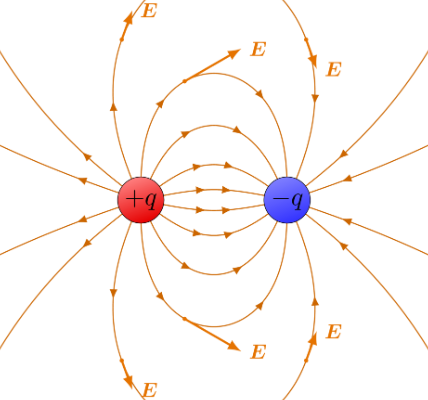
\includegraphics[scale = 0.4]{image/dipolo.png}
    \caption{campo elettromagnetico formato da un dipolo}
    \label{OndeElettrtomagnetiche}
\end{figure}

Se prendessimo un dipolo, insieme di cariche positive e negative bilanciate, e iniziassimo a muoverle esse genererebbero un campo elettrico variabile nel tempo. Dunque in ogni punto si genera un campo magnetico perpendicolare al campo elettrico. Nel caso della Figura \ref{OndeElettrtomagnetiche} ci potremmo immaginare un cerchio che esce dal foglio, e quello rappresenterebbe il campo magnetico, crea un vortice che attraversa il foglio. Questo procedimento si ripete all'infinito ed otteniamo le onde elettromagnetiche mostrate nella seguente Figura.

\begin{figure}[h]
    \centering
    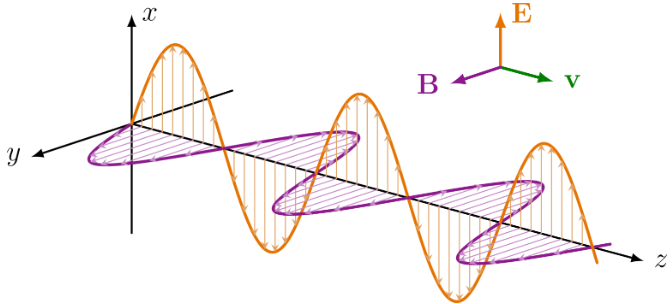
\includegraphics[scale=0.5]{image/ondeElettomagnetiche.png}
    \caption{Propagazione onde elettromagnetiche}
    \label{OndeElettromagentiche}
\end{figure}

Dal punto di vista delle equazioni non c'è un limite di frequenza delle oscillazioni ma tecnologicamente parlando si è arrivati all'ordine dei Gigahertz, un miliardo di oscillazioini al secondo.
\paragraph{}
Ora queste equazioni, per studiare le onde elettromagnetiche, si dovrebbero trasformare in equazioni differenziali perché così guardiamo cosa succede nel singolo punto e non cosa succede nell'insieme.

\section{Equazioni differenziali di Maxwell}

La trasformazione delle equazioni integrali in equazioni differenziali è possibile facendo tendere a zero il volume della superficie chiusa dove è applicato l'integrale.

\begin{equation*}
    \lim_{\Delta v \to 0}  \frac{\oint_s \vec{E} \cdot d\vec{s}}{\Delta v}  = \vec{\nabla}\cdot \vec{E}
\end{equation*}
questo limite ci da la divergenza, uno scalare il quale è la somma di tutte le componenti del gradiente, del campo elettrico. La divergenza di un campo vettoriale è la descrizione matematica
della tendenza del campo a “fuoriuscire” da un punto.

\paragraph{}
In modo analogo si trova l'equazione differenziale lungo una linea chiusa.

\begin{equation*}
    \lim_{\Delta s \to 0}  \frac{\oint_l \vec{E} \cdot d\vec{l}}{\Delta s}  = \vec{\nabla} \times \vec{E}
\end{equation*}

in questo altro caso il limite restituisce il rotore del campo elettrico. Il rotore di un campo vettoriale misura la tendenza del campo a “circolare” attorno a un punto.

\paragraph{}
Dunque le equazioni in forma differenziale diventano:

\begin{equation*}
    1)\vec{\nabla}\cdot \vec{E}  = \frac{\rho}{\varepsilon_0}\qquad3)\,\vec{\nabla} \cdot \vec{B}  = 0
\end{equation*}

\begin{equation*}
    2)\vec{\nabla} \times \vec{E}  = -\frac{d\vec{B}}{dt}\qquad4)\,\vec{\nabla} \times \vec{B}  = \mu_0 \vec{J} + \varepsilon_0\mu_0\frac{d\vec{E}}{dt}
\end{equation*}

\section{Formula di Biot-Savart o prima formula di Laplace}

Questa formula è la sorella della Formula di Coulomb, ma applicata al campo magnetico:

\begin{equation}
    \vec{B} = \frac{\mu_0}{4\pi} \frac{q\vec{v} \times \vec{Ur}}{r^2}
\end{equation}

In un dato punto: 

\begin{equation}
    d\vec{B} = \frac{\mu_0}{4\pi} \frac{i d\vec{l} \times \vec{Ur}}{r^2}
\end{equation}

\section{Filo infinito}

\begin{figure}[H]
    \centering
    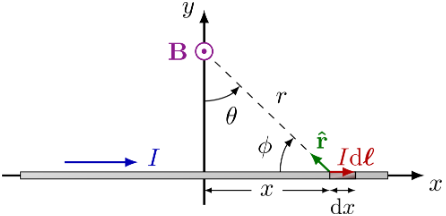
\includegraphics[scale = 0.5]{image/filoInfinitoMagnetico.png}
    \caption{Campo magnetico ad una distanza h dal filo}
    \label{campoMagneticodaUnFiloLeggeBiotSavart}
\end{figure}

\begin{equation}
    d\vec{B} = \frac{\mu_0}{4\pi} \frac{i d\vec{l} \times \vec{Ur}}{r^2}
\end{equation}

Per calcolarlo dobbiamo trasformare tutto in funzione di Theta. Quindi:

\begin{equation*}
    \frac{x}{r} = \tan{\theta}
\end{equation*}
\begin{equation*}
    x = r\tan{\theta}
\end{equation*}
\begin{equation*}
    dx = \frac{r}{\cos^2{\theta}} d\theta
\end{equation*}

\begin{equation*}
    \frac{d}{r} = \cos{\theta}
\end{equation*}
dove $d$ è la distanza dal filo.
\begin{equation*}
    r = \frac{d}{\cos{\theta}}
\end{equation*}

Quindi la formula risulta essere la seguente:

\begin{equation*}
    d\vec{B} = \frac{\mu_0}{4\pi} \frac{i d d\theta \cos{\theta}}{\cos^2{\theta}} \frac{\cos^2{\theta}}{d^2}
\end{equation*}

Semplificando e integrando:

\begin{equation}
    B = \frac{\mu_0 i}{4\pi d}\int_{-\theta} ^{\theta} \cos{\theta} d\theta
\end{equation}

dove $d$ è sempre la distanza tra il punto e il filo. Questo risultato lo avevamo già trovato servendoci della legge di Ampere, infatti se prendiamo $\theta = \frac{\pi}{2}$ avremo proprio:

\begin{equation}
    B = \frac{\mu_0 i}{2 \pi d}\
\end{equation}



Si preferisce usare questa formula perché la legge di Biot-Savart è valida su qualsiasi filo.


\section{Spira}

\begin{figure}[H]
    \centering
    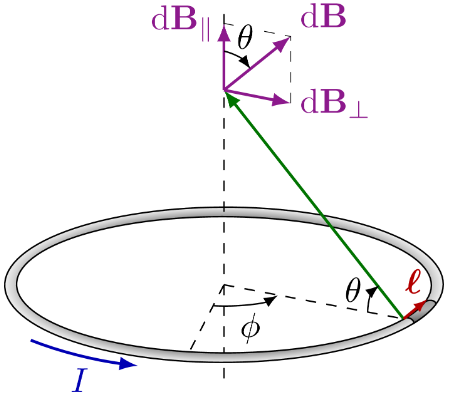
\includegraphics[scale = 0.5]{image/spira.png}
    \caption{Campo magnetico generato da una spira}
    \label{spira}
\end{figure}

\begin{equation}
    B = \frac{\mu_0 i r^2}{2(r^2 + h^2)^{\frac{3}{2}}}
\end{equation}

Dove $r$ risulta essere il raggio e $h$ l'altezza che vi è tra la spira e il punto.

\section{Applicazione della legge di Faraday}

\begin{figure}[H]
    \centering
    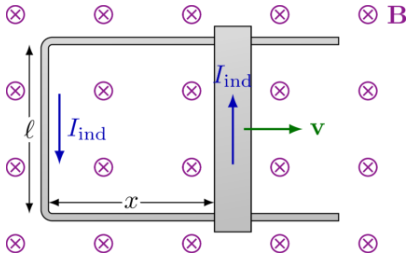
\includegraphics[scale = 0.5]{image/FaradayApplicazione.png}
    \caption{Induzione elettromagnetica}
    \label{FaradayApplicazione}
\end{figure}

Vorremmo calcolare il campo magnetico dell'area compresa tra il filo e la barra.

Per la legge di Faraday calcoliamo facilmente il flusso:

\begin{equation*}
    \oint_l \vec{E} \cdot d\vec{l}  = -\frac{d}{dt}\phi_b
\end{equation*}

dove $\phi_b = Blvt$ 

Derivandola nel tempo troviamo che:

\begin{equation}
    f.e.m.\footnote{f.e.m. = Forza ElettroMotrice, è una differenza di potenziale} = \oint_l \vec{E} \cdot d\vec{l}  = Blv
\end{equation}

L'area sta aumentando quindi il flusso di B sta aumentando, ed esso crea un campo elettrico e dunque una corrente. Tale corrente risulta essere:

\begin{equation*}
    I = \frac{f.e.m}{R}
\end{equation*}

Dove $R$ si intende la resistenza nel circuito.

Questo fenomeno si chiama \textbf{induzione elettromagnetica}.

\section{Legge di Lorentz}
Ogni carica sulla barretta viene spostata con una verta velocità $v$, quindi si genera una forza, concorde al segno della corrente e tale forza risulta essere:

\begin{equation}
    \vec{F} = qvB
\end{equation}

e dunque il lavoro di una forza risulta essere:

\begin{equation}
    L = qvBl
\end{equation}

e il lavoro per unità di carica è:
\begin{equation}
    \frac{L}{q} = Blv
\end{equation}

e risulta essere uguale proprio alla $f.e.m.$.

\section{Induttore}

\begin{figure}[H]
    \centering
    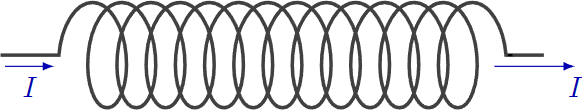
\includegraphics[scale = 0.4]{image/solenoide.png}
    \caption{Induttore}
    \label{Induttore}
\end{figure}

L'induttore è un componente elettrico che genera un campo magnetico al passaggio di corrente elettrica.

Formula principale:

\begin{equation}
    \Delta V = L \frac{dI}{dt}
\end{equation}

Ciò significa che la differenza di potenziale ai capi del solenoide risulta proporzionale ad $L$, l'induttanza, moltiplicato alla derivata nel tempo della corrente, una corrente variabile nel tempo.

Questa relazione può essere dedotta dalle equazioni di base dell'elettromagnetismo grazie alla legge di Ampere, e che abbiamo già dimostrato in precendenza:

\begin{equation}
    B = \frac{\mu_0IN}{l}
\end{equation}

dove $l$ è la lunghezza del solenoide considerato.


Se la corrente I che scorre nel solenoide/induttore è variabile nel tempo, anche B sarà variabile nel tempo. Essendo B variabile nel tempo, si produce una variazione di flusso del campo magnetico concatenato con il solenoide stesso il che produce, per la legge di Faraday, una f.e.m. auto-indotta ai capi dell'induttore, e dunque anche una differenza di potenziale tra una spira e l'altra.

\paragraph{}
Infatti per la legge di Faraday possiamo scrivere che su ogni spira si crea una differenza di potenziale:

\begin{equation*}
    -\frac{d \phi_B}{dt} = El = \Delta V
\end{equation*}
dove $l$ in questo caso è un giro della spira.

per trovare la differenza di potenziale totale, basta moltiplicarlo per il numero di spire $N$:

\begin{equation*}
    \Delta V_{tot} = N \frac{d \phi_B}{dt}
\end{equation*}
\begin{equation*}
    \Delta V_{tot} = N A \frac{\mu_0 N}{l} \frac{d I}{dt} 
\end{equation*}

dove $A$ risulta essere la sezione del tubo, $N$ il numero di spire e $l$ la lunghezza del solenoide.


$A \frac{\mu_0 N}{l}$, viene chiamata auto-induttanza o più semplicemente induttanza e si indica con L.

ecco dimostrato la legge di prima:

\begin{equation}
    \Delta V = \frac{d \phi_B}{dt} = L \frac{d I}{dt} 
    \label{eqSolenoide}
\end{equation}


Il solenoide è un parente stretto del condensatore, infatti oltre alla Equazioni \ref{equazioneCondensatore} e \ref{eqSolenoide}, che legano la corrente e la tensione, possiamo fare un discorso analogo che abbiamo già fatto per il condensatore: vogliamo capire dove va a finire l'energia elettrica che abbiamo usato per caricare l'induttore? Per carica di un induttore significa che si fa passare una corrente ai suoi capi e quando risulta costante allora al suo interno si è creato un campo magnetico costante.

\paragraph{}
Bene questa energia è stipata all'interno del area del solenoide. E da notare che in questo caso non si parla più di energia potenziale, come nel condensatore, ma bensì si parla di energia cinetica. 

\section{Circuito LC}

\begin{figure}[H]
    \centering
    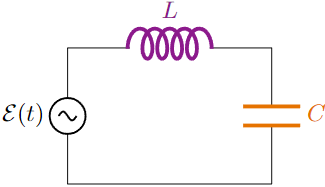
\includegraphics[scale = 0.6]{image/circuito_LC.png}
    \caption{Circuito LC}
    \label{ciruitoLc}
\end{figure}

Se creiamo un circuito formato da un induttore e da una condensatore carico otterremo un circuito risonante, perché il condensatore trasferirà tutta la sua energia, scaricandosi, all'induttore il quale si caricherà e una volta carico inizierà a ridare energia al condensatore e il ciclo riparte. Quindi questo circuito si comporta esattamente come un pendolo.
\paragraph{}
Quindi questo modo permette di creare dei clock, dei timer; ovviamente la corrente si consumerebbe nel tempo, come nel caso del pendolo, infatti si deve mantenere una tensione costante, infatti bisogna inserire anche un generatore il quale vada alla stessa frequenza con cui il circuito oscilla.

\paragraph{}
L'equazione del risonatore è:

\begin{equation}
    LC + \frac{d^2I}{dt^2} + I = 0
\end{equation}

Il risultato di questa equazione differenziale, dopo aver applicato le regole di risoluzione delle equazioni differenziali troviamo il seguente risultato:

\begin{equation}
    I(t) = I_0 \cos{\omega t}\qquad\omega = \frac{1}{\sqrt{LC}}
\end{equation}

Ovvero una corrente oscillante nel tempo.
